\documentclass{beamer}
\mode<presentation>
\usepackage{amsmath}
\usepackage{amssymb}
\usepackage{adjustbox}
\usepackage{subcaption}
\usepackage{enumitem}
\usepackage{multicol}
\usepackage{mathtools}
\usepackage{listings}
\usepackage{url}
\def\UrlBreaks{\do\/\do-}
\usetheme{Boadilla}
\usecolortheme{lily}

% Page number adjustment in footer (fixing issue)
\setbeamertemplate{footline}
{
  \leavevmode%
  \hbox{%
  \begin{beamercolorbox}[wd=\paperwidth,ht=2.25ex,dp=1ex,right]{author in head/foot}%
    \insertframenumber{} / \inserttotalframenumber\hspace*{2ex} 
  \end{beamercolorbox}}%
  \vskip0pt%
}

% Disable navigation symbols
\setbeamertemplate{navigation symbols}{}

% Define useful commands
\providecommand{\nCr}[2]{\,^{#1}C_{#2}} % nCr
\providecommand{\nPr}[2]{\,^{#1}P_{#2}} % nPr
\providecommand{\mbf}{\mathbf}
\providecommand{\pr}[1]{\ensuremath{\Pr\left(#1\right)}}
\providecommand{\qfunc}[1]{\ensuremath{Q\left(#1\right)}}
\providecommand{\sbrak}[1]{\ensuremath{{}\left[#1\right]}}
\providecommand{\lsbrak}[1]{\ensuremath{{}\left[#1\right.}}
\providecommand{\rsbrak}[1]{\ensuremath{{}\left.#1\right]}}
\providecommand{\brak}[1]{\ensuremath{\left(#1\right)}}
\providecommand{\lbrak}[1]{\ensuremath{\left(#1\right.}}
\providecommand{\rbrak}[1]{\ensuremath{\left.#1\right)}}
\providecommand{\cbrak}[1]{\ensuremath{\left\{#1\right\}}}
\providecommand{\lcbrak}[1]{\ensuremath{\left\{#1\right.}}
\providecommand{\rcbrak}[1]{\ensuremath{\left.#1\right\}}}
\theoremstyle{remark}
\newtheorem{rem}{Remark}
\newcommand{\sgn}{\mathop{\mathrm{sgn}}}
\providecommand{\abs}[1]{\left\vert#1\right\vert}
\providecommand{\res}[1]{\Res\displaylimits_{#1}} 
\providecommand{\norm}[1]{\lVert#1\rVert}
\providecommand{\mtx}[1]{\mathbf{#1}}
\providecommand{\mean}[1]{E\left[ #1 \right]}
\providecommand{\fourier}{\overset{\mathcal{F}}{ \rightleftharpoons}}
\providecommand{\system}{\overset{\mathcal{H}}{ \longleftrightarrow}}
\newcommand{\myvec}[1]{\ensuremath{\begin{pmatrix}#1\end{pmatrix}}}
\let\vec\mathbf

\lstset{
%language=C,
frame=single, 
breaklines=true,
columns=fullflexible
}

% Set section to be used in Table of Contents
\title{1-1.5-19}
\author{EE24BTECH11003 - Akshara Sarma Chennubhatla}
\date{\today} 

\begin{document}

% Title Page
\begin{frame}
\titlepage
\end{frame}

% Table of Contents (TOC)
\begin{frame}
\frametitle{Table of Contents}
\tableofcontents
\end{frame}

% Problem Statement
\section*{Problem Statement}
\begin{frame}
\frametitle{Problem Statement}
\textbf{Question:} \\Find the ratio in which the segment joining the points \brak{1,3} and \brak{4, 5} is divided by the $X$ axis. Also find the coordinates of this point on the $X$ axis.
\end{frame}

% Solution
\section{Solution}
\begin{frame}
\frametitle{Solution}
Using the section formula, the coordinates of the point dividing the line segment are given by
\begin{align}
\myvec{x\\0}&=\frac{\myvec{1\\3}+k\myvec{4\\5}}{1+k}
\end{align}
\end{frame}

\begin{frame}
\frametitle{Solution (Continued)}
Solving for \( x \), we first get
\begin{align}
\frac{5k+3}{k+1}&=0
\end{align}
\end{frame}

\begin{frame}
\frametitle{Solution (Continued)}
Solving for \( k \), we get
\begin{align}
k&=\frac{-3}{5}
\end{align}
\end{frame}

\begin{frame}
\frametitle{Solution (Continued)}
Now substituting the value of \( k \) in the equation for \( x \), we get
\begin{align}
x&=\frac{1}{k+1}+\frac{4k}{k+1}
\end{align}
\end{frame}

\begin{frame}
\frametitle{Solution (Continued)}
Simplifying the expression for \( x \), we get
\begin{align}
x&=\frac{1+4\brak{\frac{-3}{5}}}{\brak{\frac{-3}{5}}+1}
\end{align}
\end{frame}

\begin{frame}
\frametitle{Solution (Final Result)}
Finally, we obtain
\begin{align}
x&=\frac{-7}{2}
\end{align}
Therefore, the ratio in which the line segment joining the points \brak{1,3} and \brak{4,5} is divided by the $X$ axis is \( -3:5 \). The point on the $X$ axis which divides the line segment in the ratio is \brak{\frac{-7}{2}, 0}.
\end{frame}

% Plot of Points and Line
\begin{frame}
\frametitle{Plot of Points and Line}
\begin{figure}[h!]
\centering
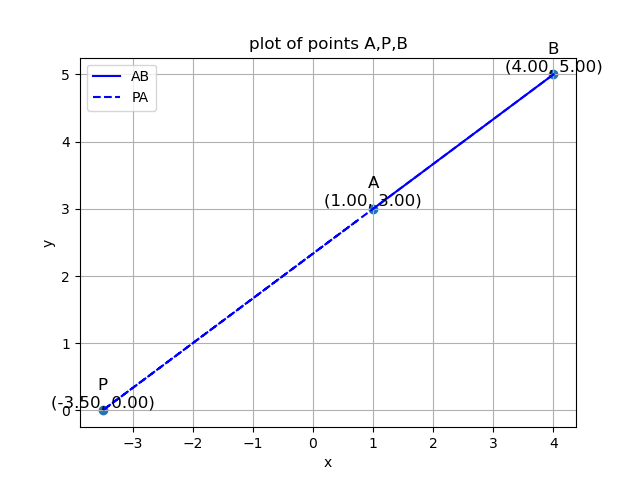
\includegraphics[width=0.7\columnwidth]{figs/figure.png}    
\caption{Plot of points A, B, and P, and the line joining them.}
\label{Plot of points A,B and P and the line joining them}
\end{figure}
\end{frame}

% C Code Section
\section{C Code}
\begin{frame}[fragile]
\frametitle{C Code (Part 1)}
\vspace{0.3cm} % Adds vertical space before the code
\begin{lstlisting}[language=C]
#include <stdio.h>
#include <stdlib.h>
#include <string.h>
#include <math.h>
#include <sys/socket.h>
#include <netinet/in.h>
#include <unistd.h>
#include "libs/matfun.h"
#include "libs/geofun.h"

void points(FILE *fptr, double **a, double **b, int num_points) {
    for (int i = 0; i <= num_points; i++) {
        double temp = (double)i/(double)num_points;
        double **output = Matadd(Matscale(a,2,1,1-temp),Matscale(b,2,1,temp),2,1);
        printf("%lf,%lf\n",output[0][0],output[1][0]);
        fprintf(fptr, "%lf,%lf\n", output[0][0], output[1][0]);
        freeMat(output,2);
    }
}
\end{lstlisting}
\vspace{0.5cm} % Adds more space after the code
\end{frame}

\begin{frame}[fragile]
\frametitle{C Code (Part 2)}
\vspace{0.3cm} % Adds vertical space before the code
\begin{lstlisting}[language=C]
int main() {
    double x1,y1,x2,y2,x3,y3;
    x1 = 1; 
    y1 = 3;
    x2 = 4; 
    y2 = 5;
    x3 = -3.5;
    y3 = 0;
    int m = 2, n = 1;
    double **A = createMat(m,n);
    double **B = createMat(m,n);
    double **P = createMat(m,n);
    A[0][0] = x1;
    A[1][0] = y1;
    B[0][0] = x2;
    B[1][0] = y2;
    P[0][0] = x3;
    P[1][0] = y3;

\begin{frame}[fragile]
\vspace{0.3cm}
    FILE *fptr;
    fptr = fopen("points.txt", "w");
    if (fptr == NULL) {
        printf("Error opening file!\n");
        return 1;
    }
\end{lstlisting} % Adds more space after the code
\end{frame}

\frametitle{C Code (Part 3)}
\vspace{0.3cm} % Adds vertical space before the code
\begin{lstlisting}[language=C]
    points(fptr, A,B ,20);
    points(fptr,P,A,20);
    fclose(fptr);
    return 0;
}
\end{lstlisting}
\vspace{0.5cm} % Adds more space after the code
\end{frame}

% Python Code Section
\section{Python Code}
\begin{frame}[fragile]
\frametitle{Python Code (Part 1)}
\vspace{0.3cm} % Adds vertical space before the code
\begin{lstlisting}[language=Python]
import numpy as np
import matplotlib.pyplot as plt
import os

# Load the points from the text file
points = np.loadtxt("points.txt", delimiter=',', max_rows=len(list(open("./points.txt")))-1)
\end{lstlisting}
\vspace{0.3cm} % Adds vertical space after the code
\end{frame}

\begin{frame}[fragile]
\frametitle{Python Code (Part 2)}
\vspace{0.3cm} % Adds vertical space before the code
\begin{lstlisting}[language=Python]
# Extract the x and y coordinates
x1 = points[:21, 0]
y1 = points[:21, 1]
x2 = points[20:, 0]
y2 = points[20:, 1]
A = np.array([1, 3]).reshape(-1,1)
P = np.array([-3.5, 0]).reshape(-1,1)
B = np.array([4, 5]).reshape(-1,1)

plt.figure()
plt.plot(x1, y1, label='AB', linestyle='-', color='blue')
plt.plot(x2, y2, label='PA', linestyle='--',color='blue')
\end{lstlisting}
\vspace{0.3cm} % Adds vertical space after the code
\end{frame}

\begin{frame}[fragile]
\frametitle{Python Code (Part 3)}
\vspace{0.3cm} % Adds vertical space before the code
\begin{lstlisting}[language=Python]
tri_coords = np.block([A,P,B])  
plt.scatter(tri_coords[0,:], tri_coords[1, :])
vert_labels = ['A','P','B'];
for i, txt in enumerate(vert_labels):
    # Annotate each point with its label and coordinates
    plt.text(tri_coords[0, i], tri_coords[1, i], f'{txt}\n({tri_coords[0, i]:.2f}, {tri_coords[1, i]:.2f})',
    fontsize=12, color = 'black', ha='center', va='bottom')
plt.xlabel("x")
plt.ylabel("y")
plt.title("plot of points A,P,B")
plt.grid(True)
plt.legend()
plt.show()
\end{lstlisting}
\vspace{0.3cm} % Adds vertical space after the code
\end{frame}

\end{document}

